\section{Gravity waves from energy}

There is an alternative derivation of the dispersion relation which is
interesting, and will be useful when the role of surface tension is
discussed in the next Section. \cite{whitham2011linear}

It begins by considering the energy of the whole system:
\[
  E := \int \left( T + U \right) d\bfr ,
\]
where the integral extends to the whole volume of the fluid, $T$ is
the total kinetic energy, and $U$ the potential energy:
\begin{align}
  T &= \frac12 \int ( \rho u^2 ) d\bfr \\
  U &=  \int (\rho \varphi) d\bfr 
\end{align}

For the simple case of gravity, the latter is simply given by
\begin{equation}
  U =    \int ( \rho g z ) d\bfr .
\end{equation}


If the flow is potential, the kinetic energy can be written as
\begin{equation}
  T = \frac12 \rho \int \left| \nabla\phi \right|^2 d\bfr ,
\end{equation}
a form that is appreciated in physics, where these sort of square
gradient theories are widely studied. (They are often called
``London-Linzburg-Landau'' theories, or a subset of those names, but
they begun, it seems, with van der Waals' seminal theory for the
liquid-vapor interface.)

In order to add more content ot our previous results, let us here
consider both an upper phase (``air'') of density $\rho'$ and a lower
one (``water'') with density $\rho$ (all primed variables refer to the
upper phase in this section). They are separated by the interfacial
surface at $z=\eta(x,y)$, but we will suppose that the surface
fluctuates around a well-defined position, which we will take, for
convenience, as $z=0$. The total potential energy is then
\[
U=
\iint dx dy   \int_{-H}^\eta  dz  ( \rho g z)
\iint dx dy   \int_\eta^{H'}  dz  ( \rho' g z)  ,
\]
where we suppose the bottom is at $z=-H$ and the air ends at $z=H'$. These
limits are not important, since we will consider later the limit
in which both are very large.

We may split the two integrals at $z=0$, the equilibrium surface:
\begin{align*}
  \iint dx dy   \int_{-H}^\eta  dz   &= 
                                       \iint dx dy   \int_{-H}^0  dz   +
                                       \iint dx dy   \int_{0}^\eta  dz   \\
  \iint dx dy   \int_\eta^{H'}  dz    &=
                                        \iint dx dy   \int_\eta^{0}  dz 
                                        \iint dx dy   \int_0^{H'}  dz  
\end{align*}

But, since two of those four integrals have fixed integration limits,
they will contribute a constant energy, so we may ignore them and just
write
\begin{align*}
  U &=\iint dx dy   \int_{0}^\eta  \rho g z  dz   -
  \iint dx dy   \int_\eta^{0} \rho' g z dz = \\
  & g  (\rho-\rho')  \iint dx dy   \int_0^{\eta} z  dz =
  \frac 12 g  (\rho-\rho')  \iint dx dy \eta^2 .
\end{align*}

It is natural that the potential energy is due to fluctiations of the
surface. However, the kinetic energy, which involves the motion of the
upper and lower fluid masses, can also be cast as a surface integral.
We may use the divergence (Gauss') theorem for this purpose. In order
to express the kinetic energy integrand as a divergence, we may write
\[
  \nabla\cdot [ \phi (\nabla \phi) ]  =
  |\nabla \phi|^2 +
  \phi \nabla^2 \phi .
\]
But the last term is null due to incompressibility. The same applies
to $\phi'$. This means the kinetic energy of the denser fluid can be
written as
\[
  T_1 = \frac12 \rho \int \nabla\cdot [ \phi (\nabla \phi) ] d\bfr \approx
  \frac12 \iint dx dy \phi (\nabla \phi) \bfe_z
\]
In this expression, we have applied Gauss theorem, and approximated
the true normal to the surface with its equilibrium value $\bhe_z$.
In other words,
\[
  T_1 = \rho 
  \frac12 \iint dx dy   \phi \frac{\partial \phi}{\partial z} 
\]
Adding the upper fluid, the total kinetic energy is
\[
  T = 
  \frac12 \iint dx dy
  \left(
    \rho \phi \frac{\partial \phi }{\partial z}
    -
    \rho'\phi'\frac{\partial \phi'}{\partial z}
  \right) ,
\]
because the outward-pointing normal of the upper phase is
approximated by $-\bhe_z$.
The appearance of those partial derivatives in the vertical direction
is appealing, because they are to be made equal to the vertical
velocity of the surface, according to boundary condition
\ref{eq:waves_bc2}.
%
Assuming a planar wave as in \ref{eq:wave_on_x}, and with our solution
for the potential in \ref{eq:wave_potential}, the necessary ingredients
are readily found:
\begin{align*}
  \frac{\partial \phi }{\partial z} &= \frac{\partial \eta }{\partial t}=
                                      a \omega \sin(kx -\omega t)  \\
  \phi(0) &= \frac{a \omega  }{ k }  \tanh(kh) \sin(kx -\omega t ) .
\end{align*}
For the upper phase, the appropriate potential is easily seen to be
\[
  \phi' = - \frac{a \omega  \cosh(k( h' - z )) }{ k \sinh( kh' )  } \sin(kx -\omega t ) ,
\]
since it must decay in the $z$ direction, satisfy the boundary
condition at $z=h'$, and the kinematic condition at the interface.

From now on, we will take the deep-water limit, leaving the general
case as an exercise to the reader. In this limit, the potentials approach
\[
  \phi(0)  = - \phi'(0) \to \frac{a \omega  }{ k }   \sin(kx -\omega t ) ,
\]
and the kinetic energy is
\[
  T = 
  \frac12 (\rho+\rho')     \frac{ (a \omega)^2  }{ k }
  \iint dx dy   \sin^2(kx -\omega t ) .
\]

For the same planar wave, the potential energy is
\[
  U = 
  \frac12 g (\rho-\rho') a^2  
  \iint dx dy   \cos^2(kx -\omega t ) .
\]

Now, the integral may be carried out: the $y$ integration yields
$L_y$, the length of the system in that direction, and on $x$ we may
have $N = L_x /\lambda $ total repetitions of the same wave, each one
of them we can integrate:
\begin{align*}
&  \iint dx dy   \cos^2(kx -\omega t ) =   \iint dx dy   \sin^2(kx -\omega t ) = \\
&  L_y N  \iint_0^\lambda dx   \cos^2(kx -\omega t ) =
  \frac12 L_y N \lambda = \frac12 A,
\end{align*}
where $A=L_x L_y$ is the total interfacial area.

This means both energies per surface area are
\[
  \frac{U}{A} = \frac14 g (\rho-\rho') a^2 \qquad
  \frac{T}{A} = \frac14 (\rho+\rho') \frac{ (a \omega)^2  }{ k } .
\]

The dispersion relation \ref{eq:water_disp_deep} is recovered (for
$\rho'=0$) if both energies are made equal. This is a tipical
requirement for oscillatory motion in physics, often called
``equipartition'' (not to be confused with a similar concept
in statistical mechanics). Its most well-known instance is the
harmonic oscillator.

A more formal justification comes from the Lagrangian%
\index{Lagrangian}.  This quantity (not to be confused with the
Lagrangian framework, or the Lagrangian derivative) is defined as
\[
  L = T - E .
\]

In classical mechanics, extremization of this quantity results in
the proper equations of motion. In our case,
\[
  \frac{L}{A} = \frac14 a^2
  \left(
    (\rho+\rho') \frac{ \omega^2  }{ k } -
    g (\rho-\rho')
  \right) .
\]

Extremization means that the partial derivatives of the Lagrangian
with respect to the parameters must be zero (technically, the
Lagrangian is not at a minimum or maximum, but at a saddle point).  In
our case, the only parameter is the amplitude, $a$, so
\[
\frac{\partial L}{\partial a} \implies 
    (\rho+\rho') \frac{ \omega^2  }{ k } -
    g (\rho-\rho') .
\]
This also implies $T=U$.

Hence, our previous deep-water dispersion relation
\ref{eq:water_disp_deep} is now modified to
\[
\omega^2  =    g  k \frac{\rho-\rho'}{\rho + \rho'}
\]

The combination $(\rho-\rho')/(\rho + \rho')$ is called the Atwood
number, and is closely $1$ when the denser fluid is much heavier than
the lighter one.


\section{Capillary waves}

The previous method can readilly accomodate capillary
waves\index{capillary waves}, also known as
``ripples''\index{ripples}. These are small waves that are dominated
by surface tension, not gravity. This is the dominant force at small
scales, and we will get an exact expression for the crossover lenght
below which this holds. Again, only the deep-water limit will be
considered.. Notice that, while this limit was bound to be violated
sooner or later for long gravity waves (when their wave-length begins
to be comparable to the water depth), capillary waves will eventually
comply with this limit at small wave-lengths.


The surface tension causes a cost in modifying an interface from its
equilibrium value:
\[
U_\mathrm{st} = \sigma (A - A_0),
\]
where $\sigma$ is the surface tension, with units of energy per area.

The area of a distorted surface in the Monge representation is given by
\[
  A = \iint dx dy \sqrt{
    1 +
    \left( \frac{\partial \eta}{\partial x} \right)^2 +
    \left( \frac{\partial \eta}{\partial y} \right)^2
  } .
\]
When fluctuation are not great, the cumbersome square root may
be expanded in Fourier series, and we find:

\begin{align*}
  A & \approx \iint dx dy 
  \left(
    1 + \frac12 \left[
      \left( \frac{\partial \eta}{\partial x} \right)^2 +
      \left( \frac{\partial \eta}{\partial y} \right)^2
    \right]
      \right) = \\
  &= A_0 + \frac12
  \iint dx dy 
  \left(
      \left( \frac{\partial \eta}{\partial x} \right)^2 +
      \left( \frac{\partial \eta}{\partial y} \right)^2
    \right)  
\end{align*}

For our perturbation \ref{eq:wave_on_x} we have,
\[
U_\mathrm{st} = \frac12   \sigma  
  \iint dx dy 
  \left( \frac{\partial \eta}{\partial x} \right)^2  =
  \frac14 \sigma A (a k)^2 ,
\]
where we have performed the same integration as in the
previous section.

Our Lagrangian is now
\[
  \frac{L}{A} = \frac14 a^2
  \left(
    \sigma  k^2 + 
    (\rho+\rho') \frac{ \omega^2  }{ k } -
    g (\rho-\rho')
  \right) .
\]

Its extreme now yields this dispersion relation:
\[
  \omega^2  =    g  k \frac{\rho-\rho'}{\rho + \rho'} +
  \frac{\sigma}{\rho+\rho'} k^3 .
\]
So we see that the short wave-length regime (high values of $k$) is
indeed dominated by a new $k^3$ term due to surface tension. The long
wave-length regime (low $k$ values) is, on the other hand, unaffected.

In order to analyze this expression, let us introduce reduced units
once more,
\[
\omega=\omega_0 \omega^* \qquad k = k_0 k^* ,
\]
where the typical angular frequency and wave vector are found by
demanding this simple expression holds:
\[
\omega^{*2}= k^* + k^{*3} .
\]

After some algebra, we find
\begin{align}
  \label{eq:capillary_k0}
  k_0&=\sqrt{\frac{ g (\rho-\rho') }{ \sigma }} \\
  \label{eq:capillary_om0}
  \omega_0^2 = g  \frac{ \rho-\rho' }{ \rho + \rho' } k_0
\end{align}


Now, the reduced phase velocity is given by
\[
  c^* := \frac{\omega^*}{k^*} =
  \sqrt{\frac{1}{k^*} +  k^* } ,
\]
so that it goes from a $\sim 1/\sqrt{k} $ growth at small $k$ (this is
the gravity regime) to a $\sim \sqrt{k} $ growth at high $k$ (surface
tension regime). It therefore has a minimum at some crossover
wave-vector $k_\mathrm{cross}$, which we may find by
\[
\frac{\partial c^* }{\partial k^*} = 0 .
\]

It is actually easier to differenciate $c^{*2}$. The value is found at
$k^*_\mathrm{cross} = 1$, at which
\[
c^*_\mathrm{cross} = \sqrt{2} .
\]

The values of $k_\mathrm{cross} $ are given by bringing back the
dimension factors in \ref{eq:capillary_k0} and \ref{eq:capillary_om0}.
The velocity is given by the factor
\[
  c_0 = \frac{\omega_0}{k_0} =
  \frac{[\sigma g (\rho-\rho')]^{1/4}}{(\rho-\rho')^{1/2}} .
\]

For water and air in standard conditions,
$\sigma=\SI{70}{\milli\joule\per\meter\squared}$,
and we find
\[
  k_\mathrm{cross} = \SI{374}{\radian\per\meter} \implies
  \lambda_\mathrm{cross} = \frac{2\pi}{k_\mathrm{cross}}=
  \SI{1.7}{\centi\meter} ,
\]
and
\[
  c_\mathrm{cross} =  \SI{23}{\centi\meter\per\second} .
\]
This is the scale below wich surface tension is important, and the
phase velocity is the lower possible.

The group velocity is defined as
\[
  c_\mathrm{gr} := \frac{\partial \omega }{\partial k}  .
\]
Notice that, by differenciating $c = \omega / k$ with respect to $k$
it is easy to prove the identity:
\[
  c_\mathrm{gr} =  c + k \frac{\partial c }{\partial k}  .
\]
This clearly shows that the a difference in the values of the two
velocities is caused by dispersion: the phase velocity having a
dependence on the wave vector, as evident in the $dc/dk$ term. This
also shows that at the crossover velocity, where this term vanishes,
both velocities are the same. These waves are, then the only
non-dispersive ones possible in the deep-water regime.

The expression for the group velocity is, in reduced units,
\[
  c^*_\mathrm{gr} :=  \frac{1+ k ^2}{2\sqrt{k + k^3} } .
\]
It then goes from a low-$k$ regime in which $c_\mathrm{gr} \to c /2 $
(gravity) to a high-$k$ regime with $ c_\mathrm{gr} \to 3 c /2 $
(surface tension). In the latter regime, the group velocity is $50\%$
faster than the phase velocity.  In
\ref{fig:gravity_capillary_dispersion_k} we plot both velocities as
functions of the reduced wave-vector. Both are seen to cross at a
value of $1$.  In Figure \ref{fig:gravity_capillary_dispersion_lambda}
the same is plotted as a function of wave-length. The crossing takes
place at the reduced wave-length value of $\lambda^*=2\pi$.

\begin{figure}
  \centering
  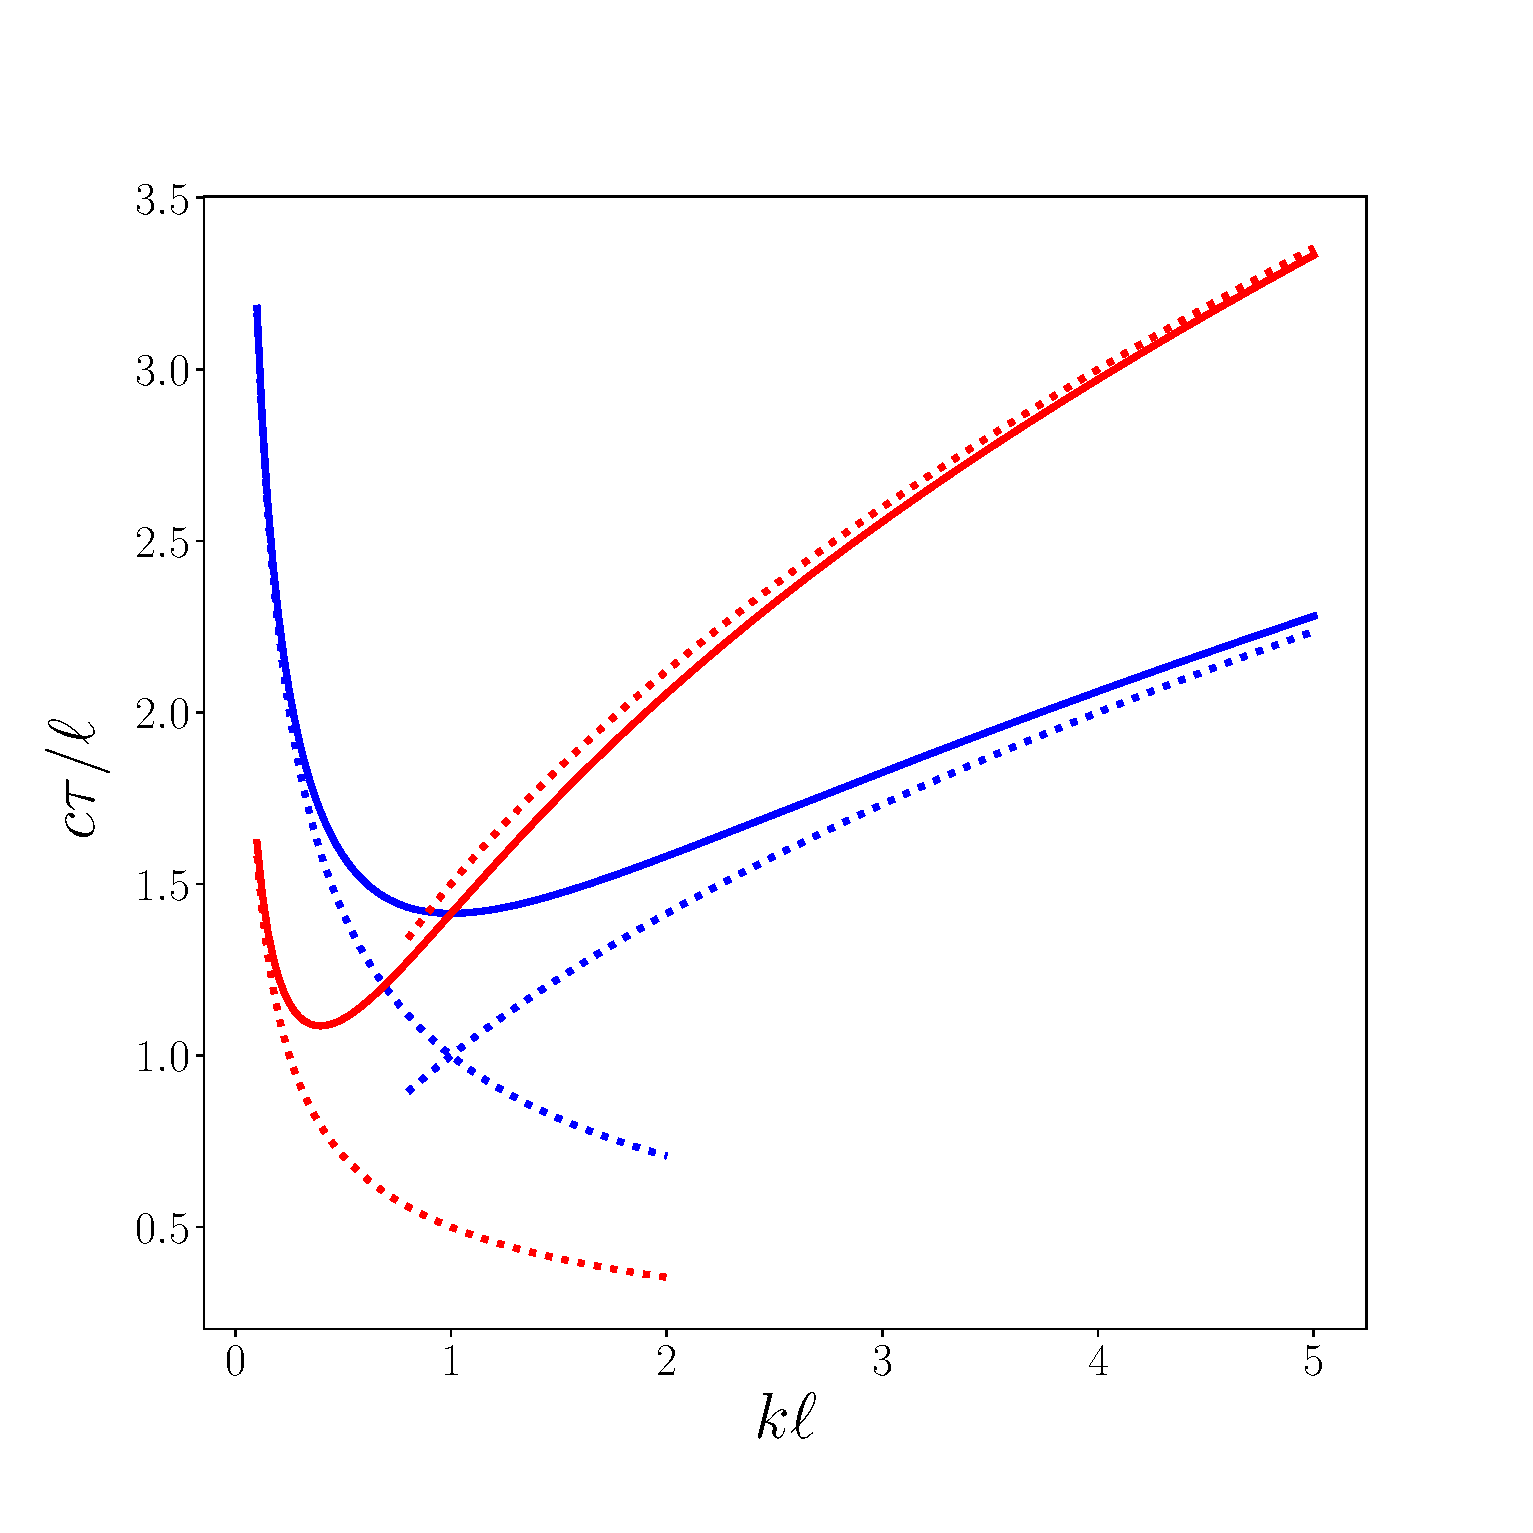
\includegraphics[width=0.4\linewidth]{figures/gravity_capillary_dispersion_k}
  \caption{\label{fig:gravity_capillary_dispersion_k}}
\end{figure}


\begin{figure}
  \centering
  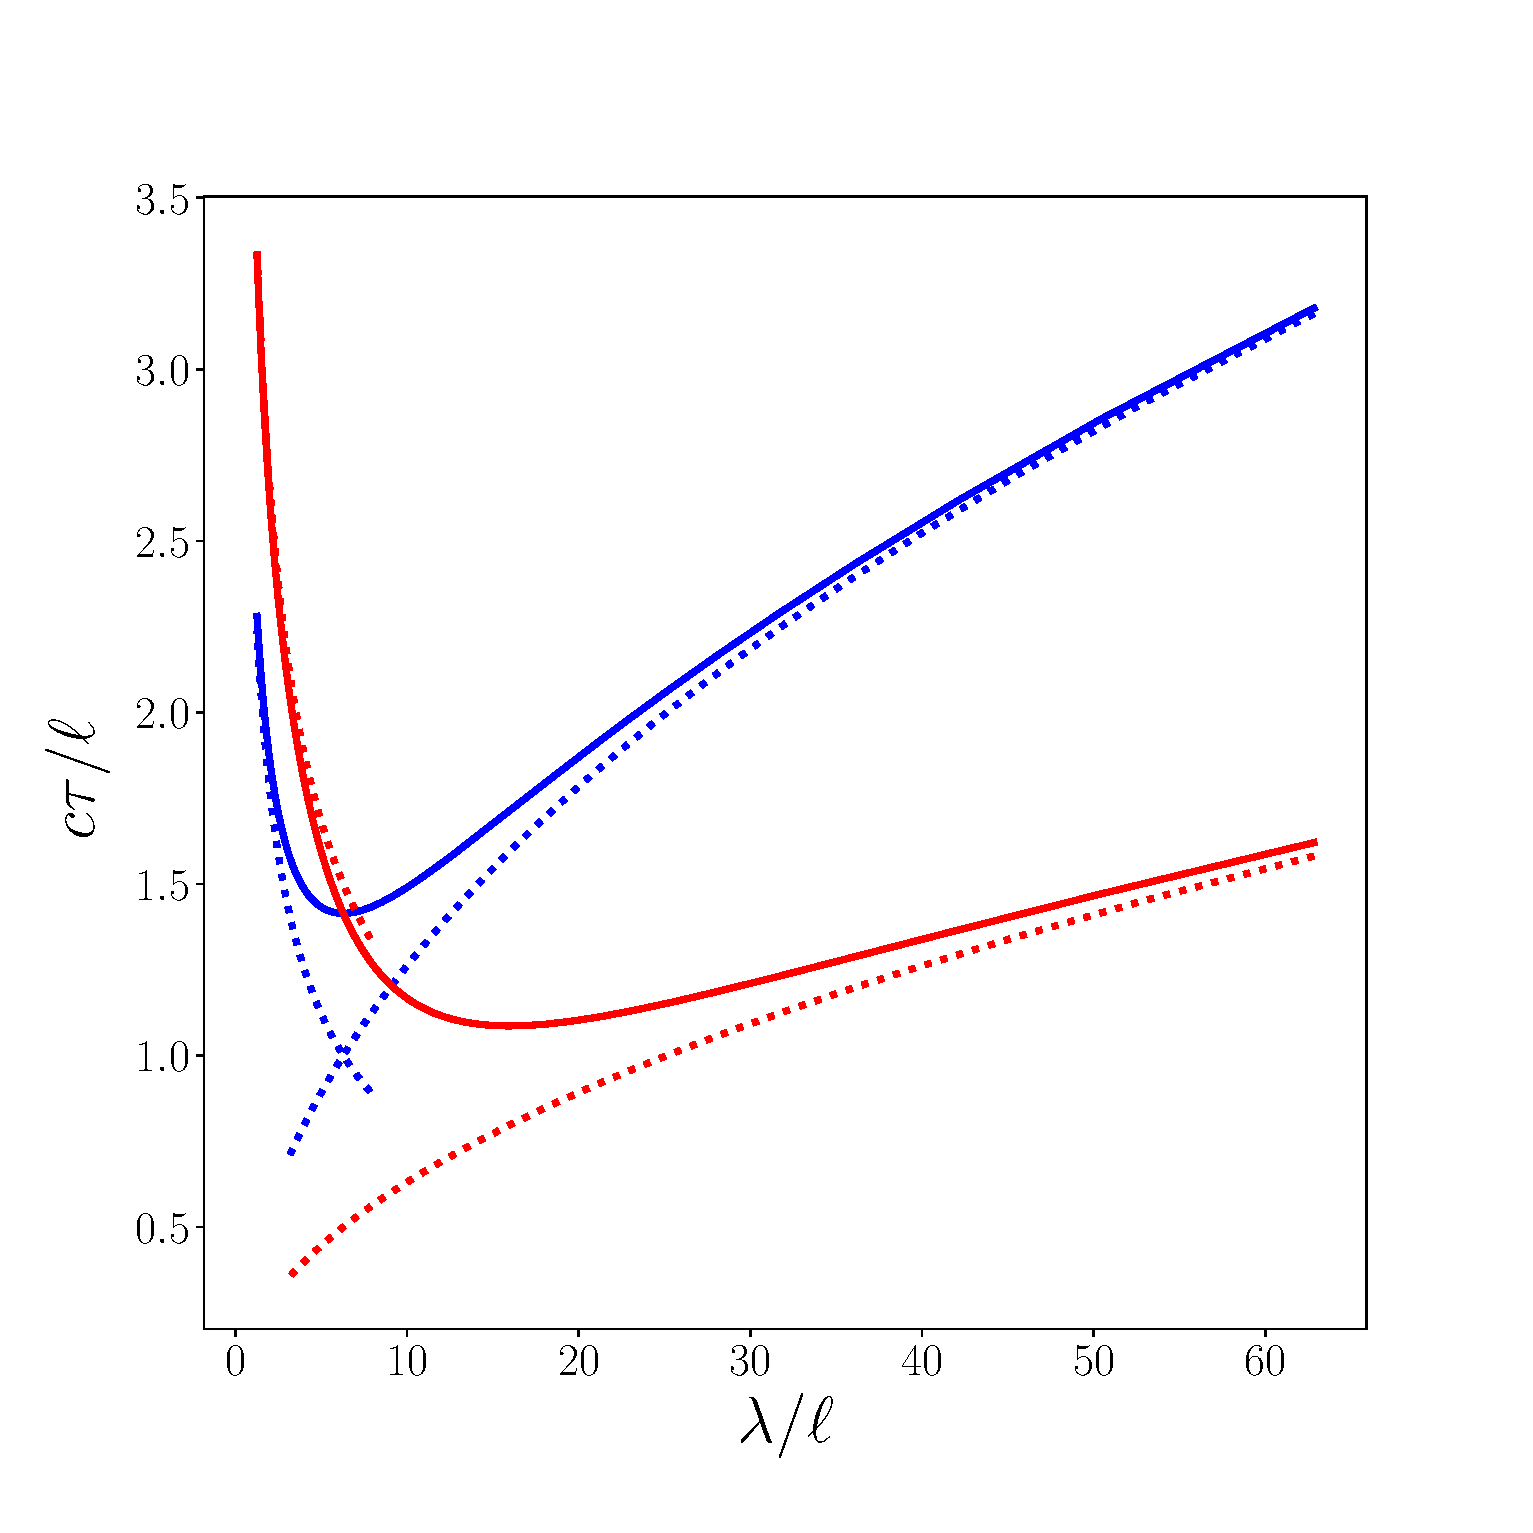
\includegraphics[width=0.4\linewidth]{figures/gravity_capillary_dispersion_lambda}
  \caption{\label{fig:gravity_capillary_dispersion_lambda}}
\end{figure}

